\section{Results and reflection}
\label{chapter:results}
\subsection{Pre-processing}
To evaluate whether or not our graph reduction technique works, we have used nine different datasets. These datasets vary between 34 and well over a million vertexes. The amount of edges varies between 78 to almost 3 million edges. There's also a significant variety in the ratio between edges and vertexes. At the low end, the edges-to-vertexes ratio is around 1.3, while the highest ratio is above 20. Figure \ref{fig:datasets} gives an overview of the different datasets.

\begin{figure}[H]
\begin{center}
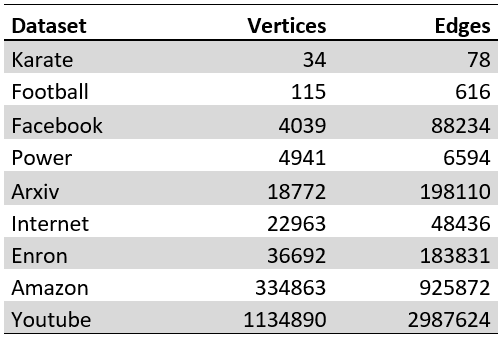
\includegraphics[width=0.5\textwidth]{images/datasets.png}
\caption{The variety of datasets used to test the algorithms}\label{fig:datasets}
\end{center}
\end{figure}

Figure \ref{fig:reducedtable} shows the results from the pre-processing algorithm. Since the algorithm uses random sampling, each graph was reduced five times and the results were averaged. The results were surprisingly good. Of the 9 graphs, 6 were reduced by around 30\% or more, while 3 were reduced by more than half both in nodes and in edges. The Internet and Power graphs did not see a lot of reduction. We believe this is due to the fact that they are graphs of internet relays and electricity relays respectively. These are inherently bound by geographic limitations, making it unlikely that large cliques form. For the YouTube dataset the reason is not immediately clear.

\begin{figure}[H]
\begin{center}
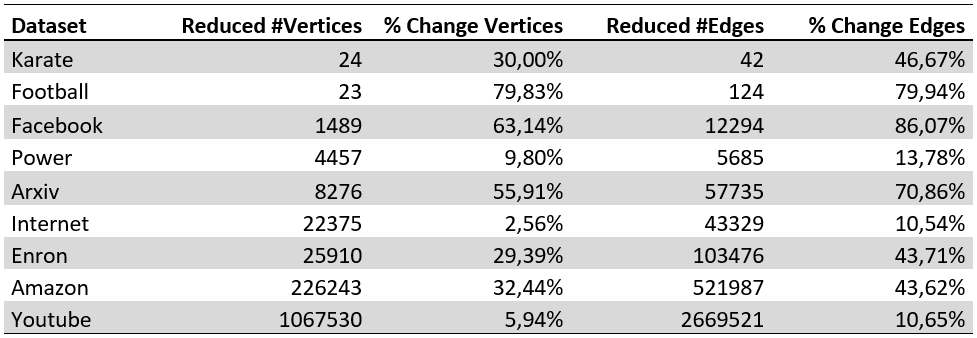
\includegraphics[width=1\textwidth]{images/reducedtable.png}
\caption{The amount of vertices and edges after the preprocessing step, as well as the percentage change.}\label{fig:reducedtable}
\end{center}
\end{figure}

The pre-processing algorithm is only useful if it doesn't take more time to run than the time it saves later on. After some iterating to solve performance issues, figure \ref{fig:prespeed} shows the average execution time to reduce each graph. The sampling method is clearly very fast, since even graphs with tens of thousands of vertexes can be processed in just a few seconds. Even the large YouTube dataset with over a million vertexes takes just under 10 minutes to process. These times are negligible compared to however long the community detection step will take on larger graphs. Another observation is that the graphs in which few cliques were found (Power and Internet) also take less time to process.

\begin{figure}[H]
\begin{center}
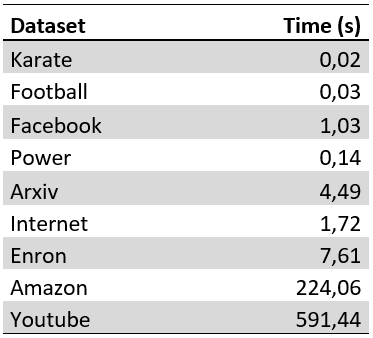
\includegraphics[width=0.4\textwidth]{images/prespeed.png}
\caption{The average execution time needed for the preprocessing step.}\label{fig:prespeed}
\end{center}
\end{figure}

\subsection{Community detection}
!!!TODO!!! algorithm settings !!!TODO!!!
To test the effects of reducing the graph, we ran the community detection genetic algorithm ten times for each graph, five times with the original graph and five times with a reduced graph. Execution time was limited to five minutes. The reported execution times and modularity scores are the averages of those five runs. The maximum execution time is only checked at the end of each generation, which is why the reported execution time can be significantly higher than five minutes. We have also noted the fitness score for a random community partitioning as a comparison. These are the average of 100 random partitionings for regular and reduced graphs. This provides a baseline measure to compare the results against.
\par
During testing we found that the self-learning operator took a very long time to complete compared to the other operators. This made generations take a very long time on larger graphs. Since we were mainly interested in the effects of reducing the graph, we disabled the self-learning operator for larger graphs. We have also repeated our tests for the smaller graphs without this operator. Results without the self-learning operator are marked with ``-SL''.\footnote{We believe this is mainly due to the slow initialization of the jenetics library. In the paper by Li and Liu, they do not seem to have this issue. }
\par
Even with the reduced graphs, the Amazon and YouTube graphs were still too large to solve in a reasonable amount of time. The Enron dataset was just barely possible, but we had to increase the maximum time to 10 minutes per run, and reduce the population size from 25 to 9.




karate: 
-slightly worse than regular due to bad clique, can search complete search space ==> larger minimum clique size? trade-off vs speed?
-performance similar
-SL much slower, slightly better results
- much better than baseline, regular has slight edge in baseline

football:
- performance edge for clique, slightly better result
- SL: regular better but much slower: SL causes premature convergence with clique
- much better than baseline, clique has slight edge in baseline

facebook:
-best case scenario
-clique is much faster and much better result
-SL for regular takes a very long time, worse result! only 2-3 gens --> SL too slow to add anything
-SL also very slow for clique, but the result is slightly better.
- huge baseline advantage for clique

power:
- only around 10\% reduction in graph, still almost twice as fast for a similar score.
- slight edge for clique baseline

arxiv:
- another best case scenario
- huge advantage for clique both in time and score
- both are just slightly above random --> algo needs more time to work (only around 30 gens)
- huge advantage for clique is due to baseline

internet:
- bad case
- clique only slightly better
- baselines almost identical

enron:
-similar to arxiv
- better result for clique, due to better baseline
- both only slightly above baseline

genetic algorithm can't do anything meaningful in 5/10 minutes for arxiv and up, advantage for clique is due to better initialization. Still good result!

Large graphs: effect of bad cliques offset by huge increase in speed.... Definitely could be a useful step for heavily interconnected graphs
